\documentclass[12pt,reqno,a4paper,oneside]{report}

\usepackage{amsfonts, amsmath,
	        amssymb, amsthm}  % Fontes e símbolos matemáticos da AMS.
\usepackage{graphicx}         % Importação de gráficos.
\usepackage[brazil]{babel}    % Idioma português (Brasil) como padrão.
\usepackage[utf8]{inputenc}   % Codificação UTF-8.
\usepackage{natbib}           % Para citações.

\usepackage{bm}          % Equações em negrito com qualidade superior.
\usepackage{booktabs}    % Edição de linhas de tabelas.
\usepackage{caption}     % Edição do texto dos títulos de tabelas.
\usepackage{color}       % Edição de cores.
\usepackage{indentfirst} % Indentará sempre o 1º parágrafo de cada seção do relatório.
%\usepackage{enumitem}   % Edição mais elaborada de listas
                         % Conflito com ambiente "enumerate"!.
%\usepackage{hyperref}   % Criação de "hyperlinks".
\usepackage{multirow}    % Para obter uma célula com uma coluna e várias linhas.
\usepackage{ragged2e}    % Opções de alinhamento do texto.
\usepackage{titlesec}    % Formatação de títulos de seções.

\usepackage[FIGTOPCAP]{subfigure}

\usepackage[top=2cm, bottom=2cm,
            left=2cm, right=2cm]{geometry} % Margens do texto.

\titleformat{\chapter}[display]
    {\normalfont\huge\bfseries}{\chaptertitlename\ \thechapter}{10pt}{\large}
\titlespacing*{\chapter}{0pt}{0pt}{15pt}

\titleformat{\section}
{\normalfont\bfseries\normalsize}
{\thesection.}{0.5em}{}

\captionsetup{justification = centering} %Centraliza os títulos das tabelas.

% Símbolo matemático para independência entre variáveis aleatórias:

\newcommand\indep{\protect\mathpalette{\protect\independenT}{\perp}}\def\independenT#1#2{\mathrel{\rlap{$#1#2$}\mkern2mu{#1#2}}}

\begin{document}

\title{\huge Relatório do Trabalho de\\
	Estatística Bayesiana I}
\author{\\
	\huge Mistura de Normais\\
	\huge com Variância Contaminada
	\\
	\\
	\\
	\\
	\Large Caio Balieiro\\
	\Large Taiguara Melo Tupinambás\\
	\Large Walmir dos Reis Miranda Filho\\
	\\
	\\
	\\
	\Large Prof. Dani Gamerman\\
	\Large Profª Rosangela Helena Loschi\\
	\\
	\\
	\\
	Programa de Pós-Graduação em Estatística\\
	Instituto de Ciências Exatas\\
	Universidade Federal de Minas Gerais\\
	\\
	\\}
\date{Belo Horizonte, 2 de dezembro de 2019}
\maketitle

\section*{\Large Introdução}

%Texto descrevendo o modelo de mistura de normais com variância contaminada (referenciando possivelmente alguns dos artigos consultados) e os objetivos do trabalho.


Considere uma amostra $X = (X_{1}, X_{2}, ..., X_{n})$ independente e identicamente distribuída da seguinte mistura finita de distribuições normais:


\begin{equation}\label{eq:dist_amostral}
f(x|\mu,\sigma^2,\nu)=\nu\phi(x|\mu,100\sigma^2)+(1-\nu)\phi(x|\mu,\sigma^2), x\in\mathcal{R}
\end{equation}

Onde $\phi(x|M,V)$ denota a função densidade de probabilidade da distribuição normal com média M e variância V avaliada no ponto $x,\mu\in\mathcal{R},\sigma^2\in\mathcal{R^+}"$ e $\nu\in(0,1)$.

\begin{itemize}
	\item Assuma que, \textit{a priori}, $\mu|\sigma^2\sim{N}(m,V\sigma^2),\sigma^2\sim{GI}(a,d)$ e $\nu\sim{U}(0,1)$. Encontre a expressão da densidade $a posteriori$ de ($\mu$,$\sigma^2$,$\nu$).
	\item Escolha valores apropriados para ($\mu$,$\sigma^2$,$\nu$). Fixado estes parâmetros, gere uma amostra de tamanho n = 500 da distribuição amostral. Armazene estes valores para análises posteriores. Faça uma apresentação gráfica apropriada da amostra gerada. Determine a média, variância, curtose e assimetria da amostra gerada.
\end{itemize}

DICA: pode-se usar, sem provar, que a mistura finita de distribuições normais pode ser hierarquicamente representada por 

$X_i|\mu,\sigma^2,U_{i}=u_i\sim{N}(\mu,\sigma^2u_i^{-1})$ e $U_i|\mu\sim{discreta}(1,100)$, com $P(U_i=100)=\nu$.

\subsection*{Escolha dos Parâmetros \textit{a priori}}


\begin{figure}[!htb]
	\centering
	\subfigure[]{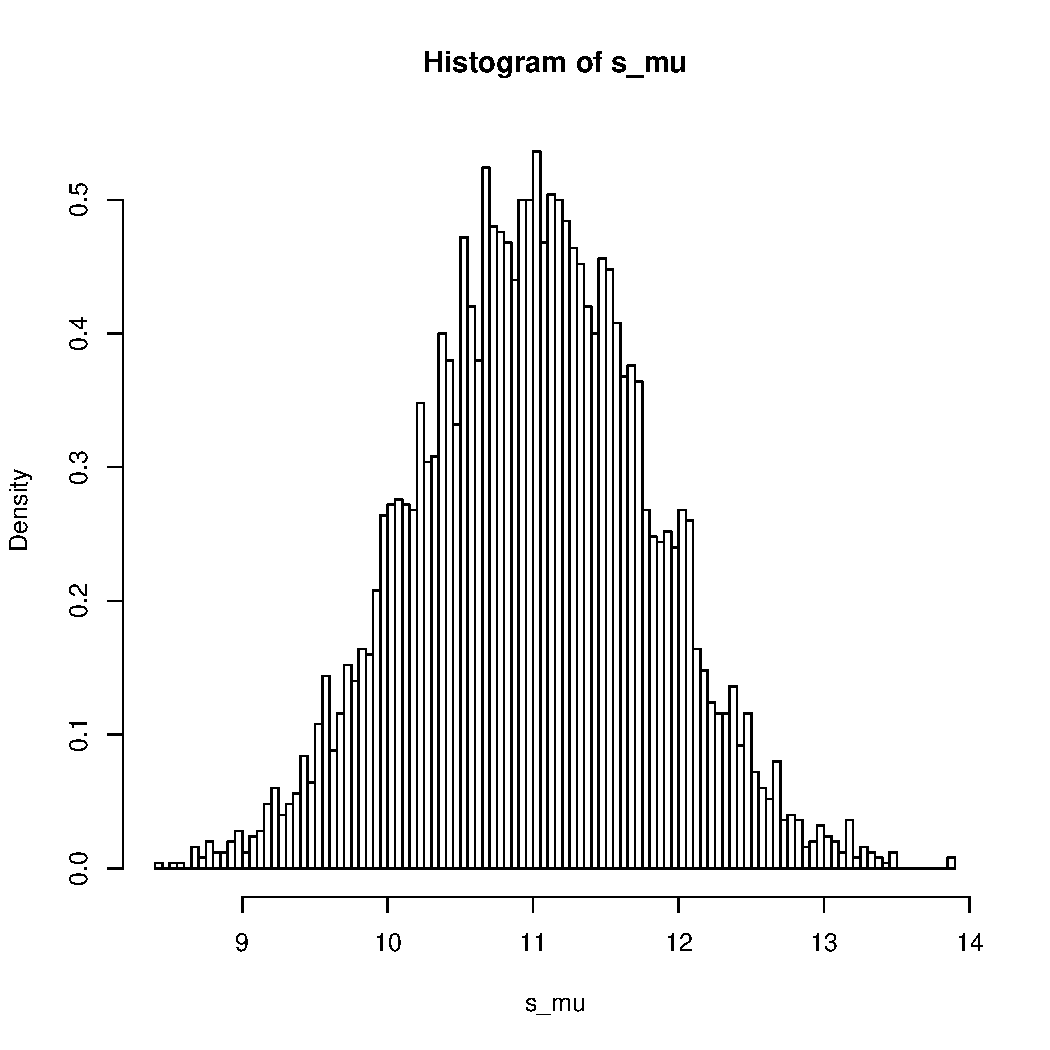
\includegraphics[width=0.45\textwidth]{figuras/parte1/priori_mu.pdf}}
	\subfigure[]{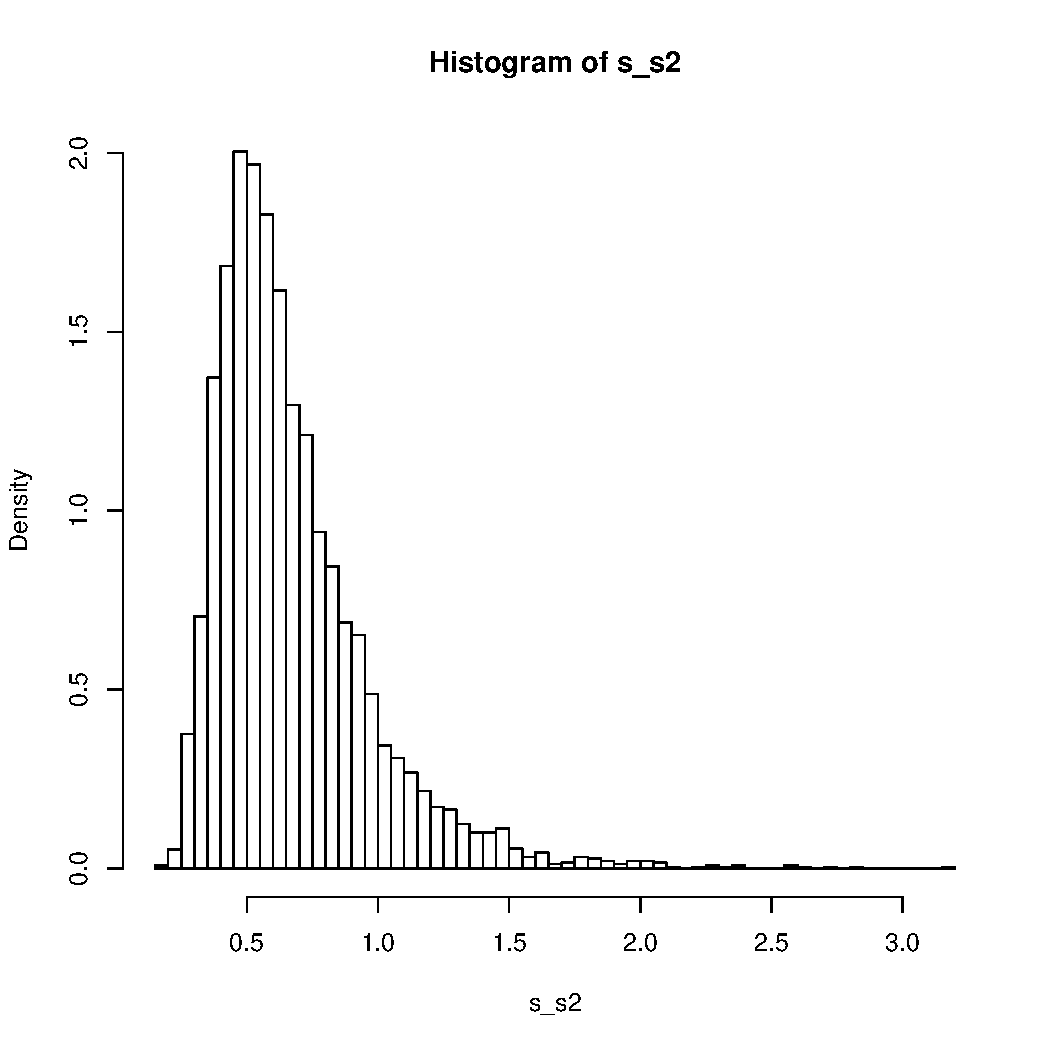
\includegraphics[width=0.45\textwidth]{figuras/parte1/priori_sigma.pdf}} 
	\caption{Distribuições a priori}
	\label{fig:priori}
\end{figure}

\begin{figure}[!htb]
	\centering
	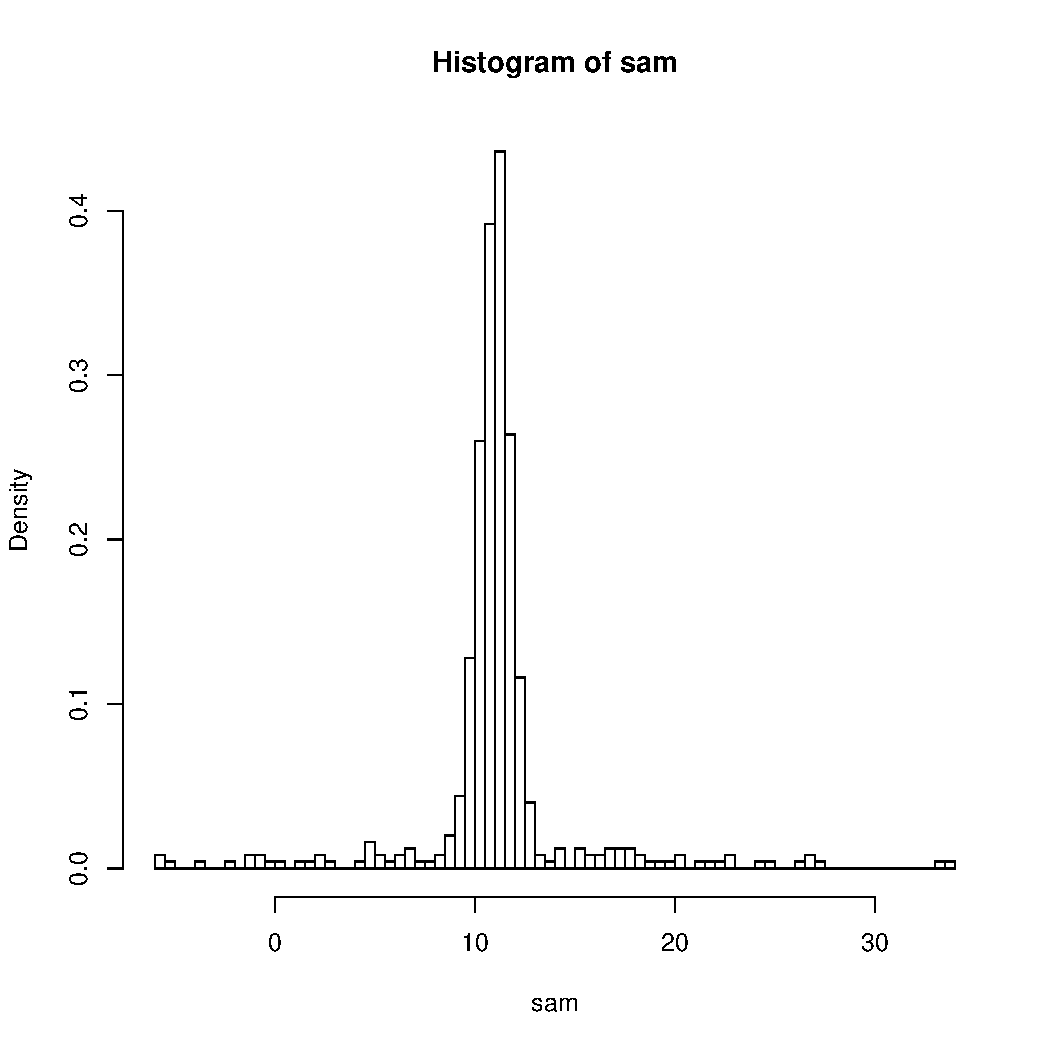
\includegraphics[width=0.75\textwidth]{figuras/parte1/amostra_n.pdf}
	\caption{Amostra de tamanho 500.}
	\label{fig:sample}
\end{figure}



\section*{\Large O Método da Quadratura de Riemann}
%Texto descrevendo o método e como foi feita neste trabalho a aproximação via quadratura de Riemann.

\begin{figure}[!htb]
	\centering
	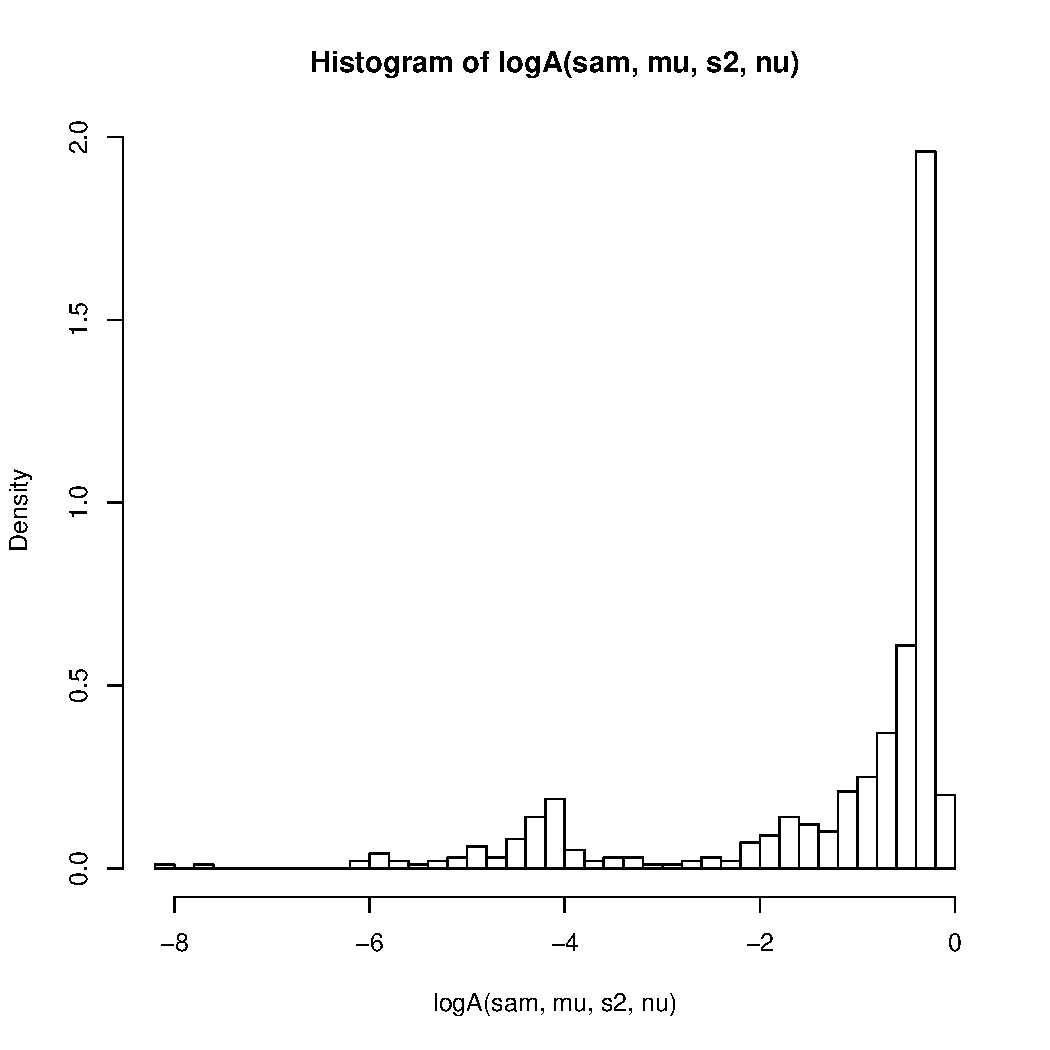
\includegraphics[width=0.75\textwidth]{figuras/parte1/logA.pdf}
	\caption{Amostra de tamanho 500.}
	\label{fig:logA}
\end{figure}

\begin{figure}[!htb]
	\centering
	\subfigure[]{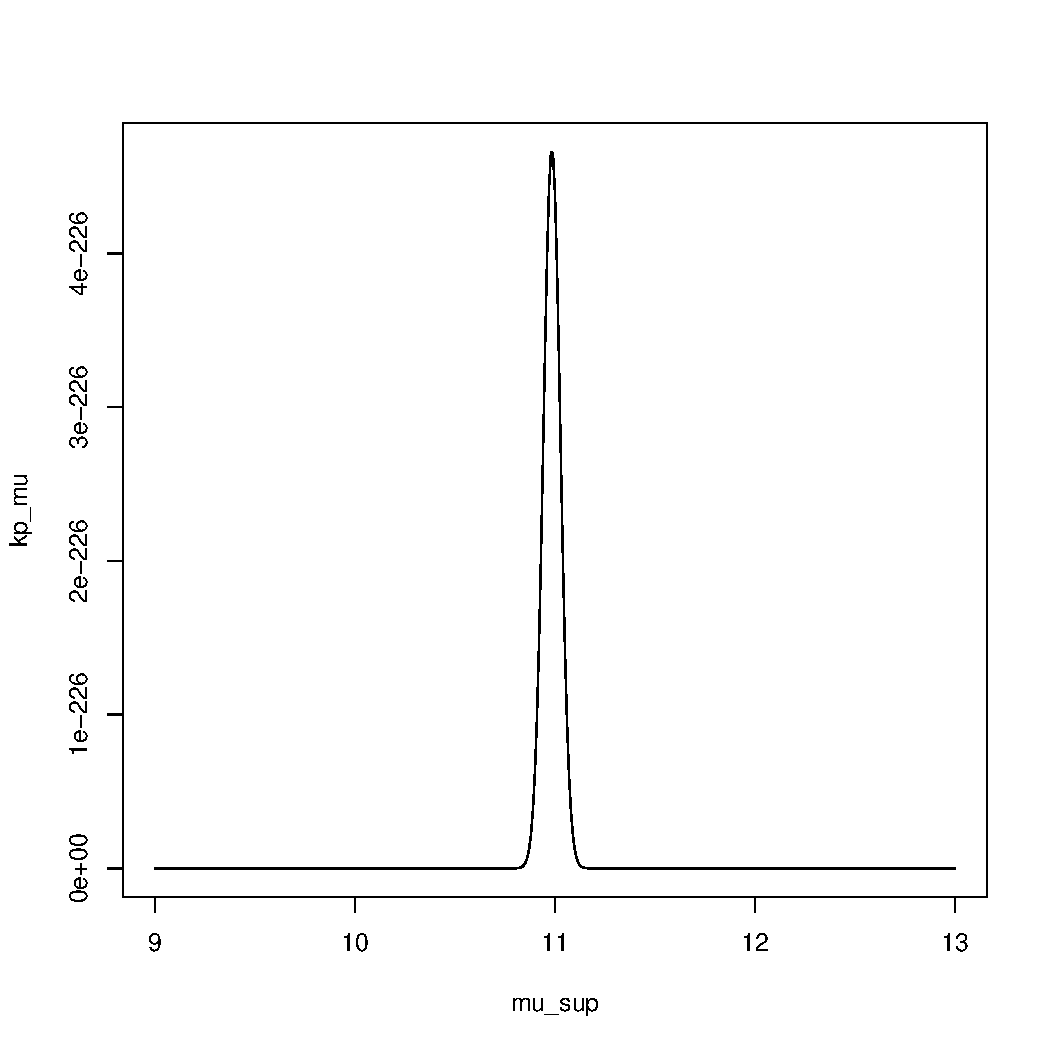
\includegraphics[width=0.45\textwidth]{figuras/parte1/grid_mu1.pdf}}
	\subfigure[]{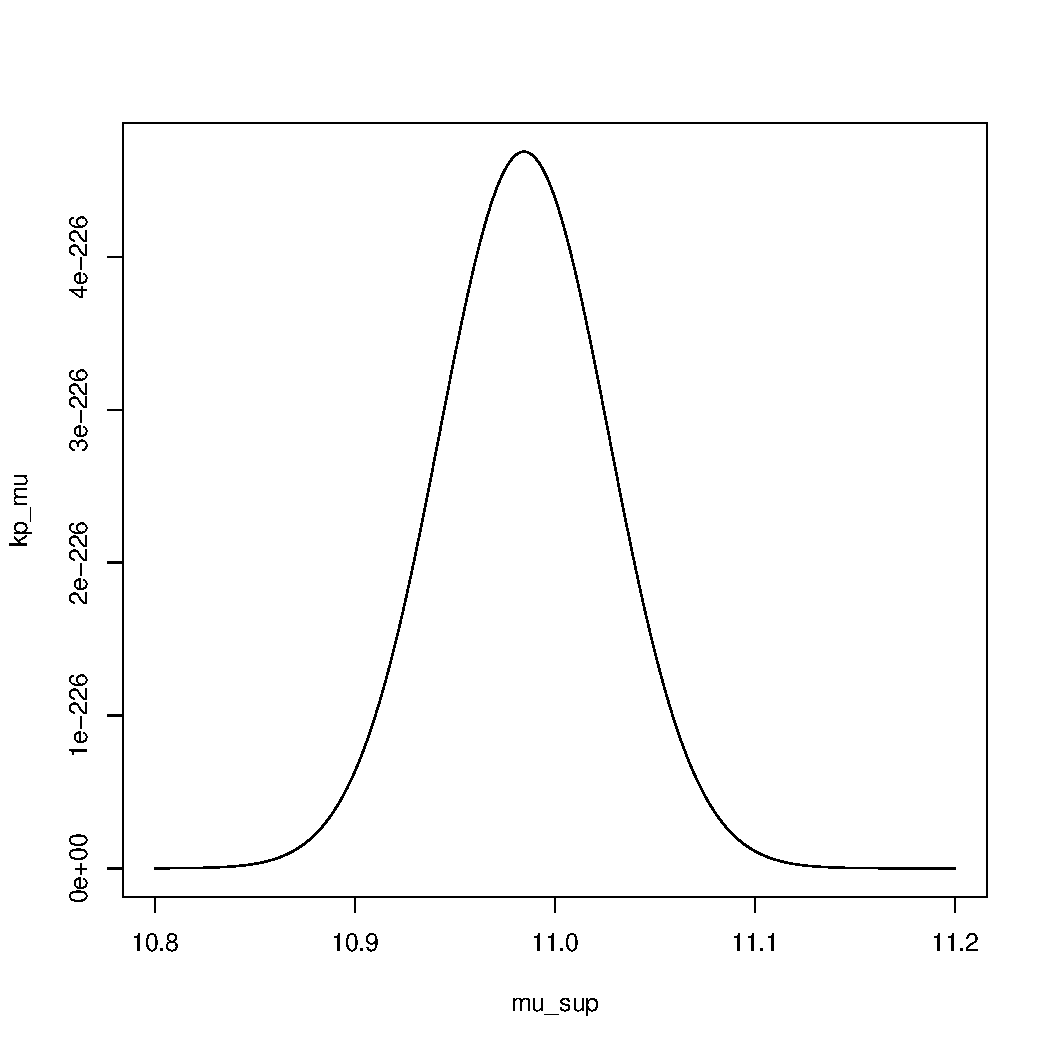
\includegraphics[width=0.45\textwidth]{figuras/parte1/grid_mu2.pdf}} 
	\caption{Grade de mu}
	\label{fig:grid_mu}
\end{figure}

\begin{figure}[!htb]
	\centering
	\subfigure[]{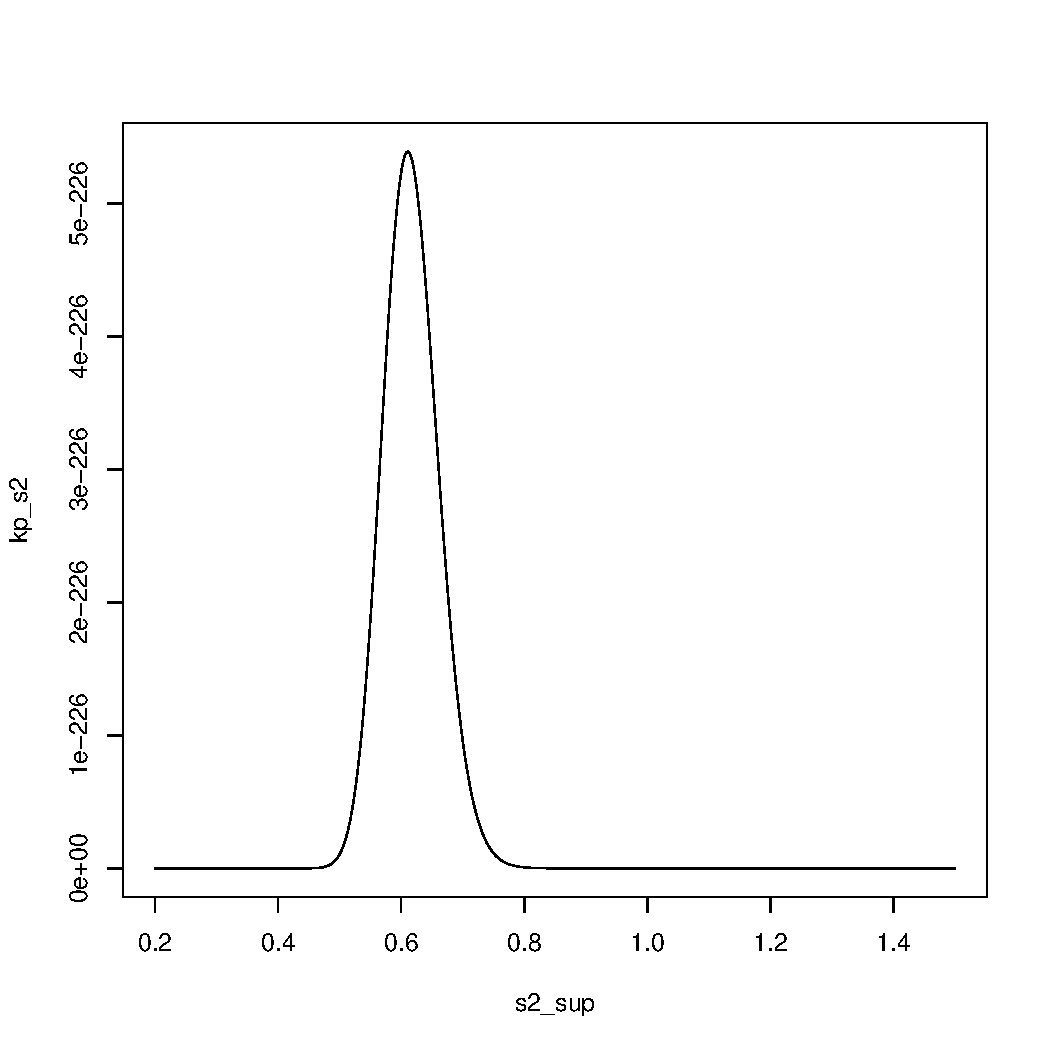
\includegraphics[width=0.45\textwidth]{figuras/parte1/grid_sigma1.pdf}}
	\subfigure[]{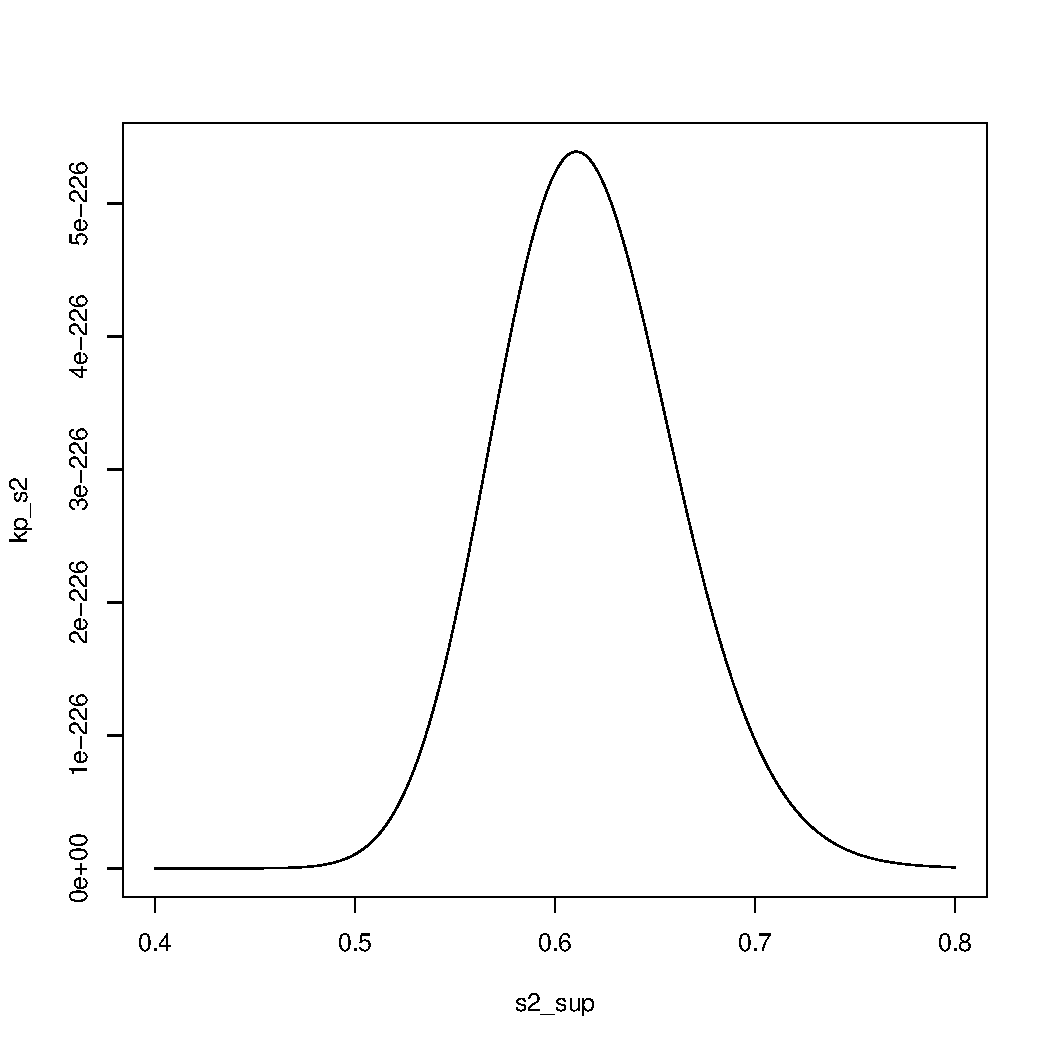
\includegraphics[width=0.45\textwidth]{figuras/parte1/grid_sigma2.pdf}} 
	\caption{Grades de sigma}
	\label{fig:grid_sigma}
\end{figure}

\begin{figure}[!htb]
	\centering
	\subfigure[]{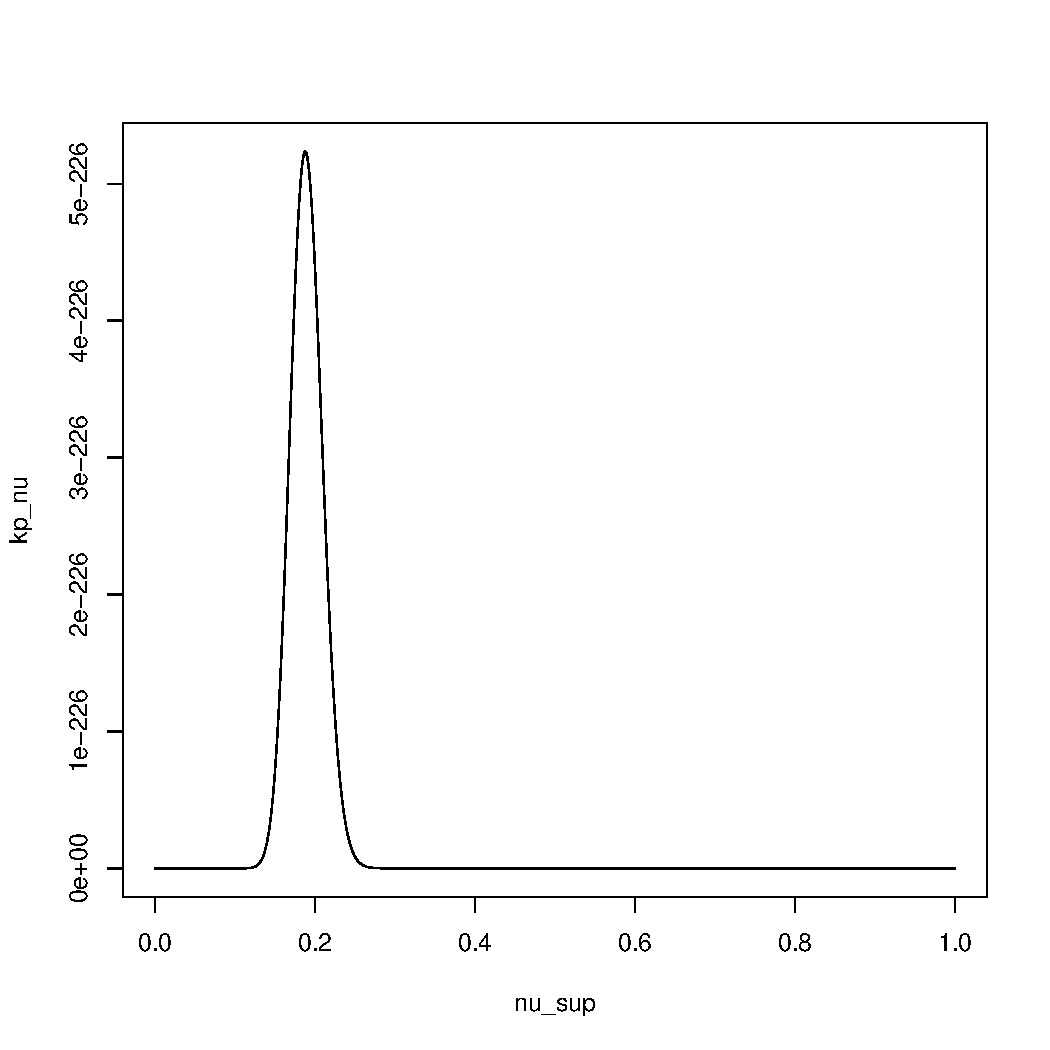
\includegraphics[width=0.45\textwidth]{figuras/parte1/grid_nu1.pdf}}
	\subfigure[]{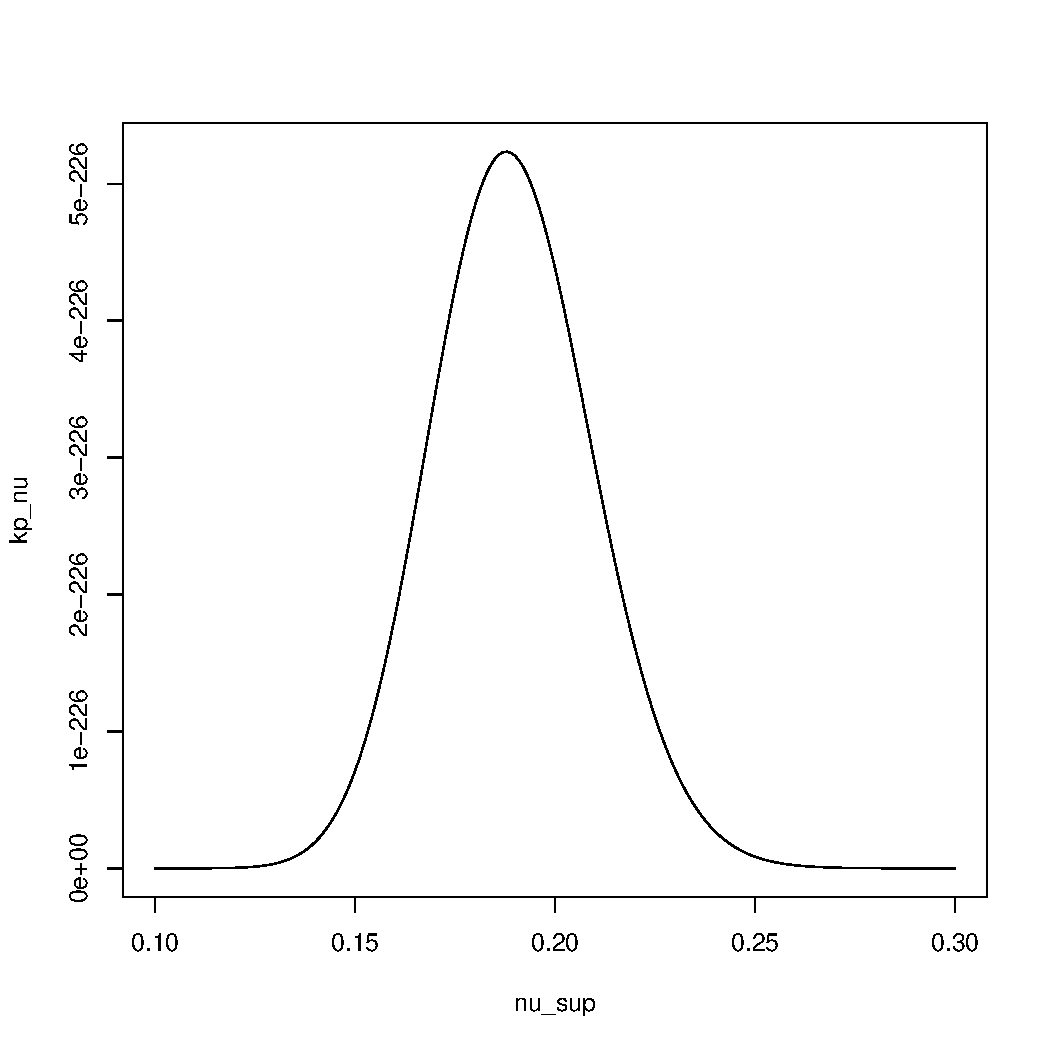
\includegraphics[width=0.45\textwidth]{figuras/parte1/grid_nu2.pdf}} 
	\caption{Grades de nu}
	\label{fig:grid_nu}
\end{figure}


\begin{figure}[!htb]
	\centering
	\subfigure[]{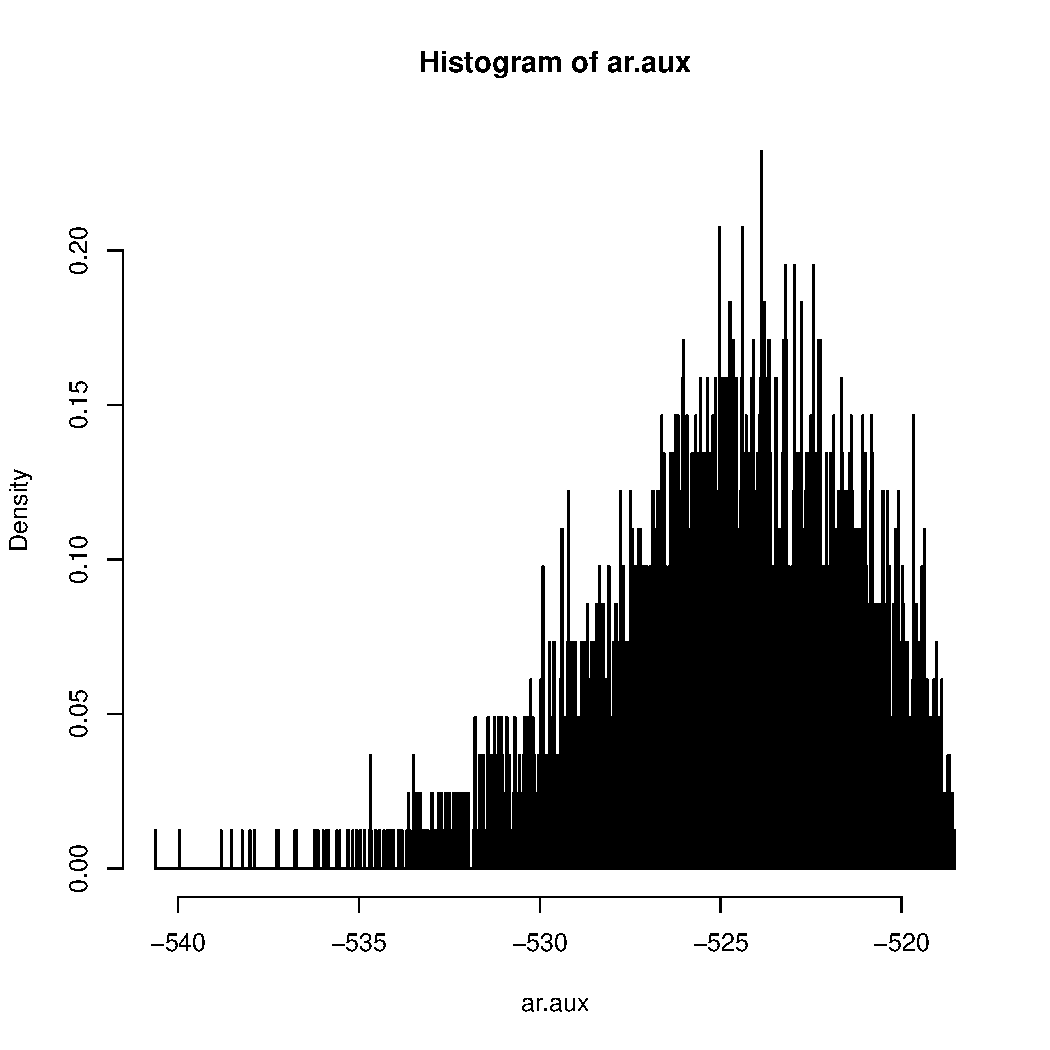
\includegraphics[width=0.3\textwidth]{figuras/parte1/constante_prop_16.pdf}}
	\subfigure[]{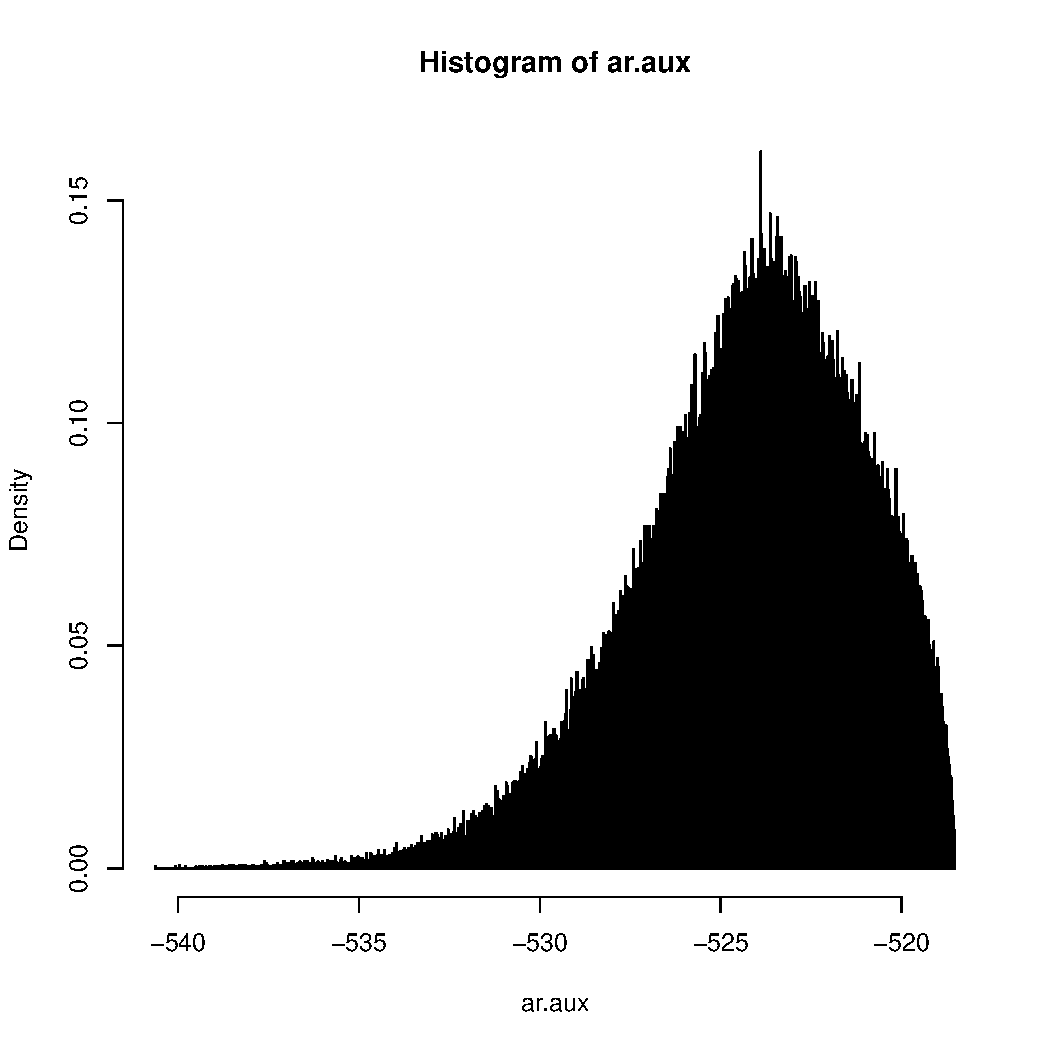
\includegraphics[width=0.3\textwidth]{figuras/parte1/constante_prop_51.pdf}} 
	\subfigure[]{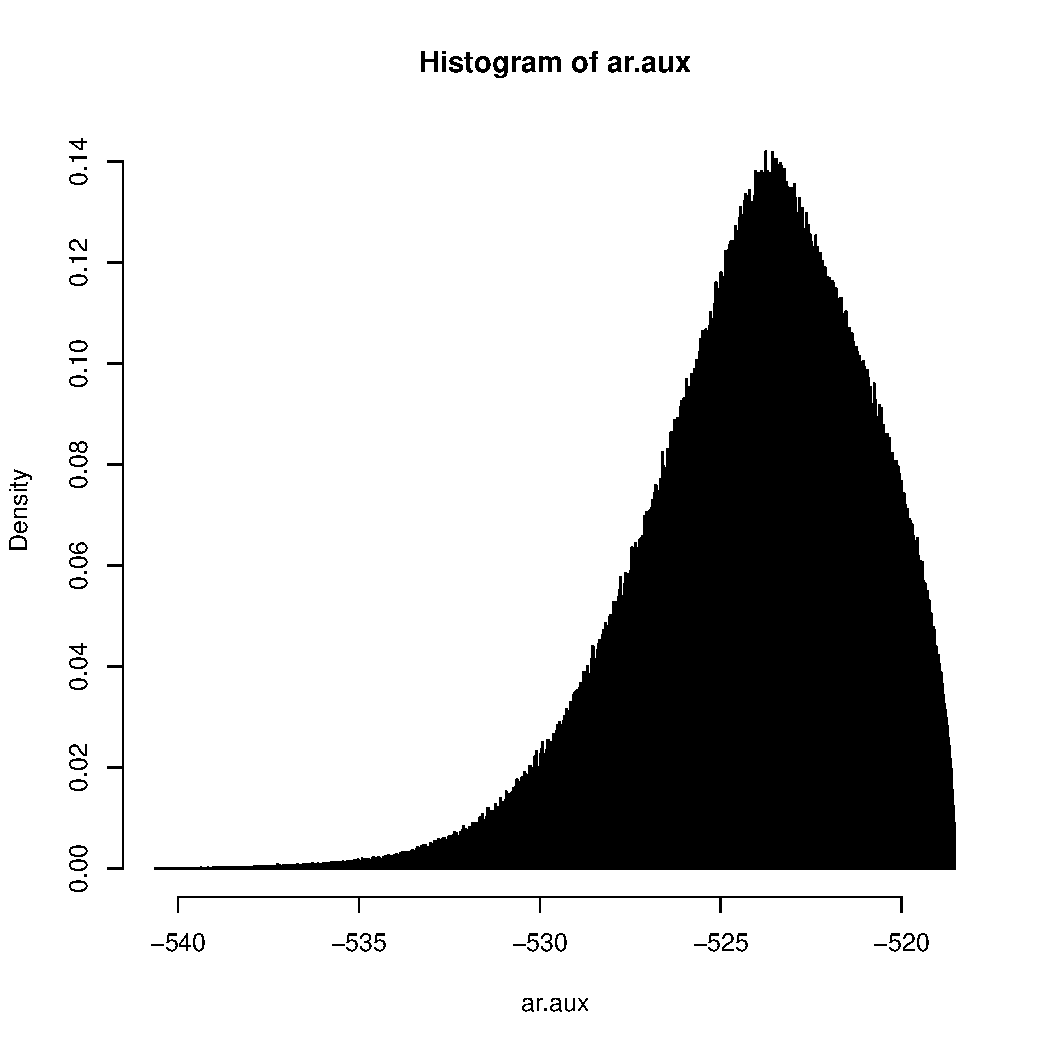
\includegraphics[width=0.3\textwidth]{figuras/parte1/constante_prop_101.pdf}} 
	\caption{Calculo da constante de proporcionalidade}
	\label{fig:const_prop}
\end{figure}


\begin{figure}[!htb]
	\centering
	\subfigure[]{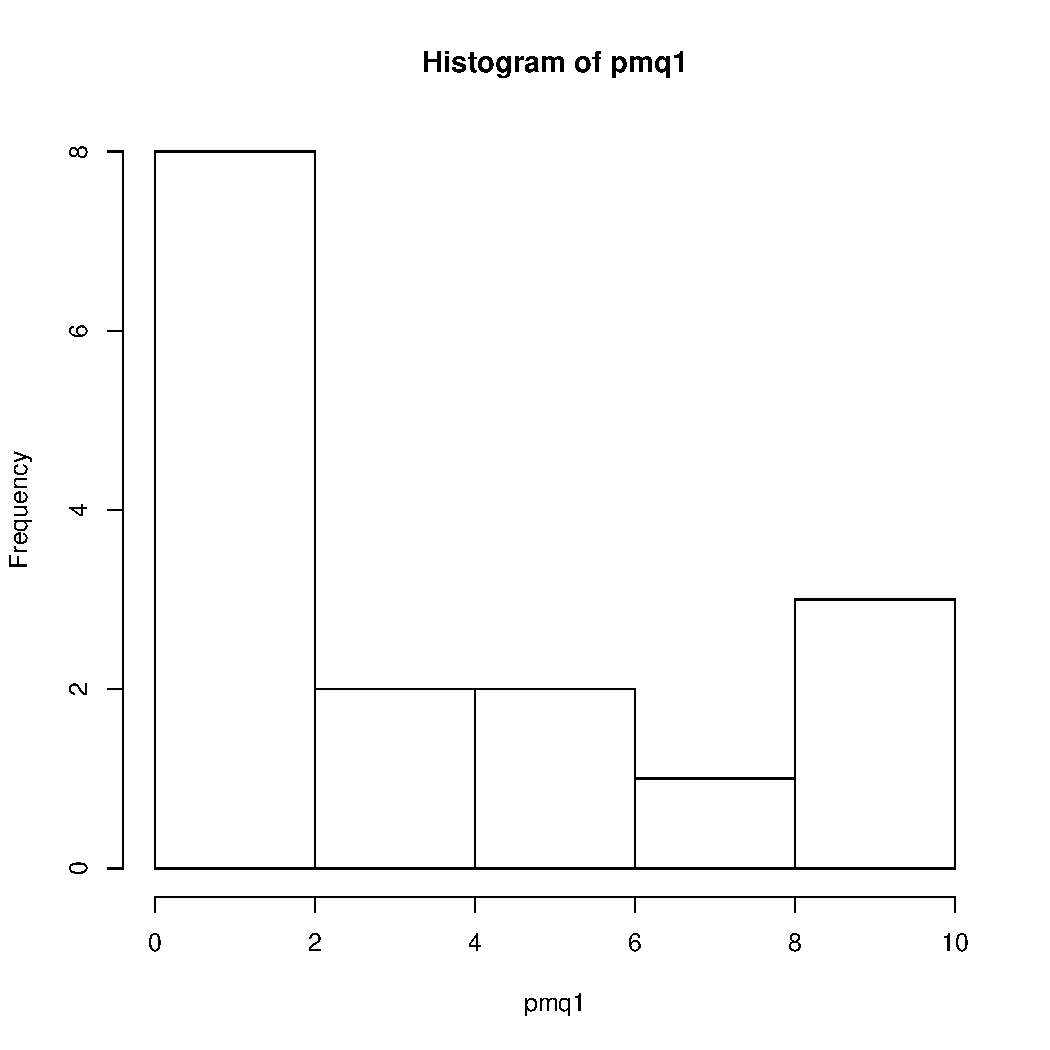
\includegraphics[width=0.3\textwidth]{figuras/parte1/post_mu1.pdf}}
	\subfigure[]{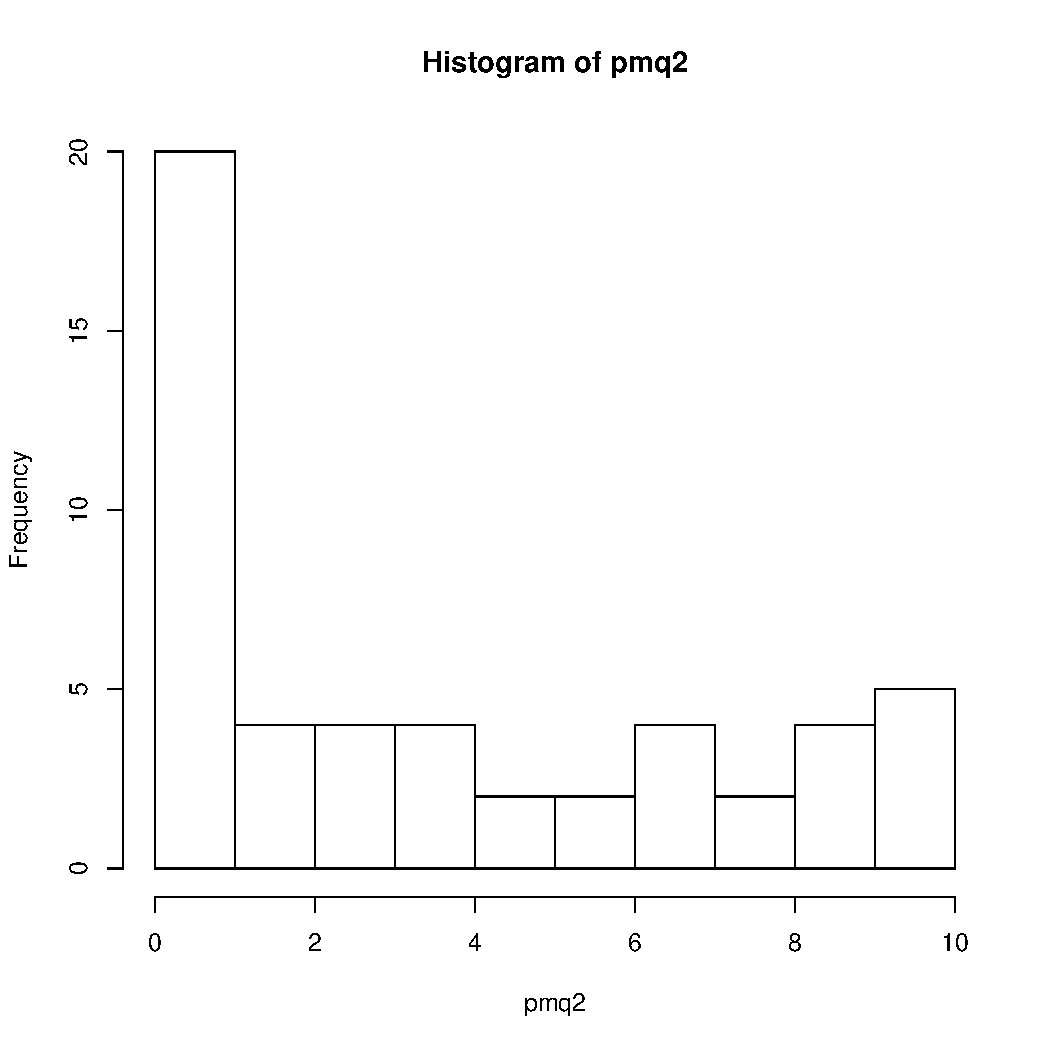
\includegraphics[width=0.3\textwidth]{figuras/parte1/post_mu2.pdf}} 
	\subfigure[]{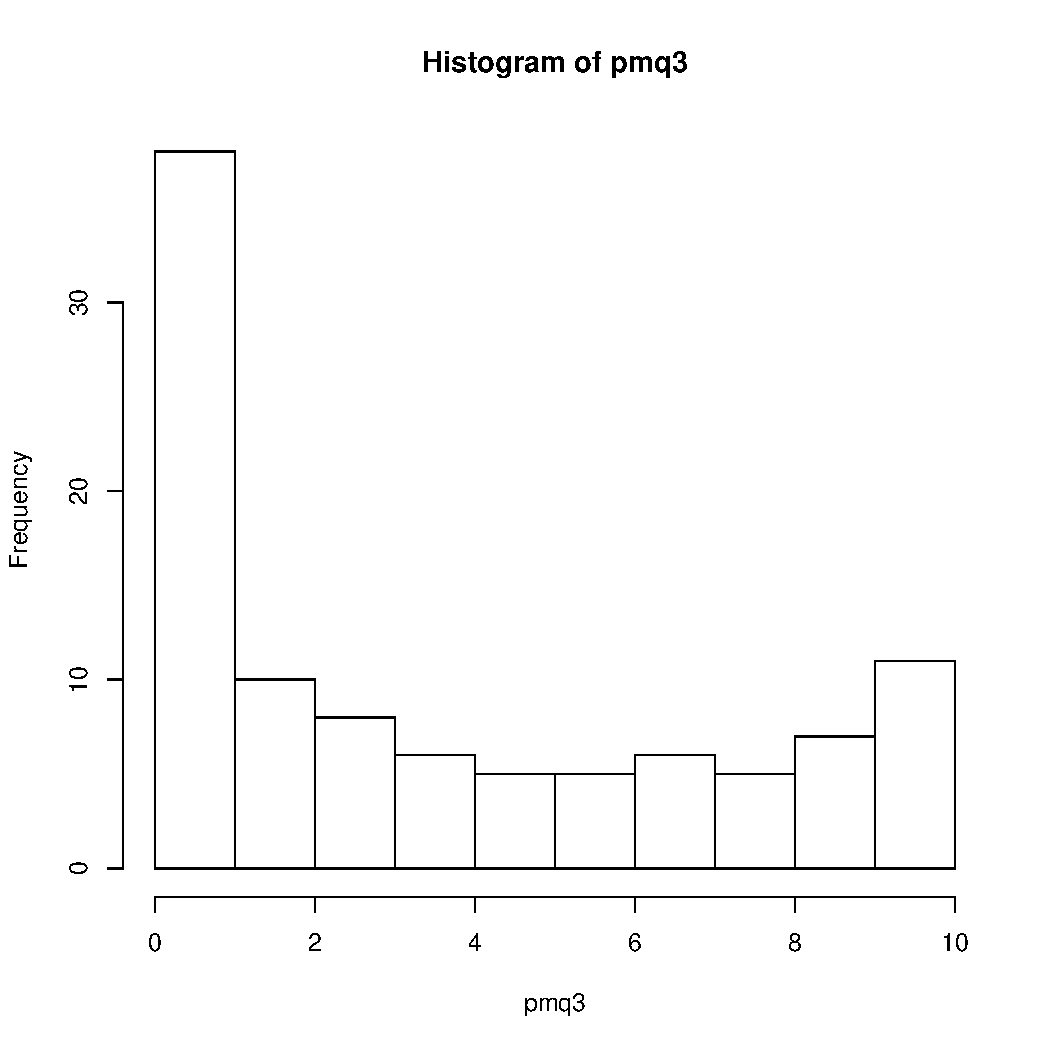
\includegraphics[width=0.3\textwidth]{figuras/parte1/post_mu3.pdf}} 
	\caption{Posteriori de mu}
	\label{fig:post_mu}
\end{figure}

\begin{figure}[!htb]
	\centering
	\subfigure[]{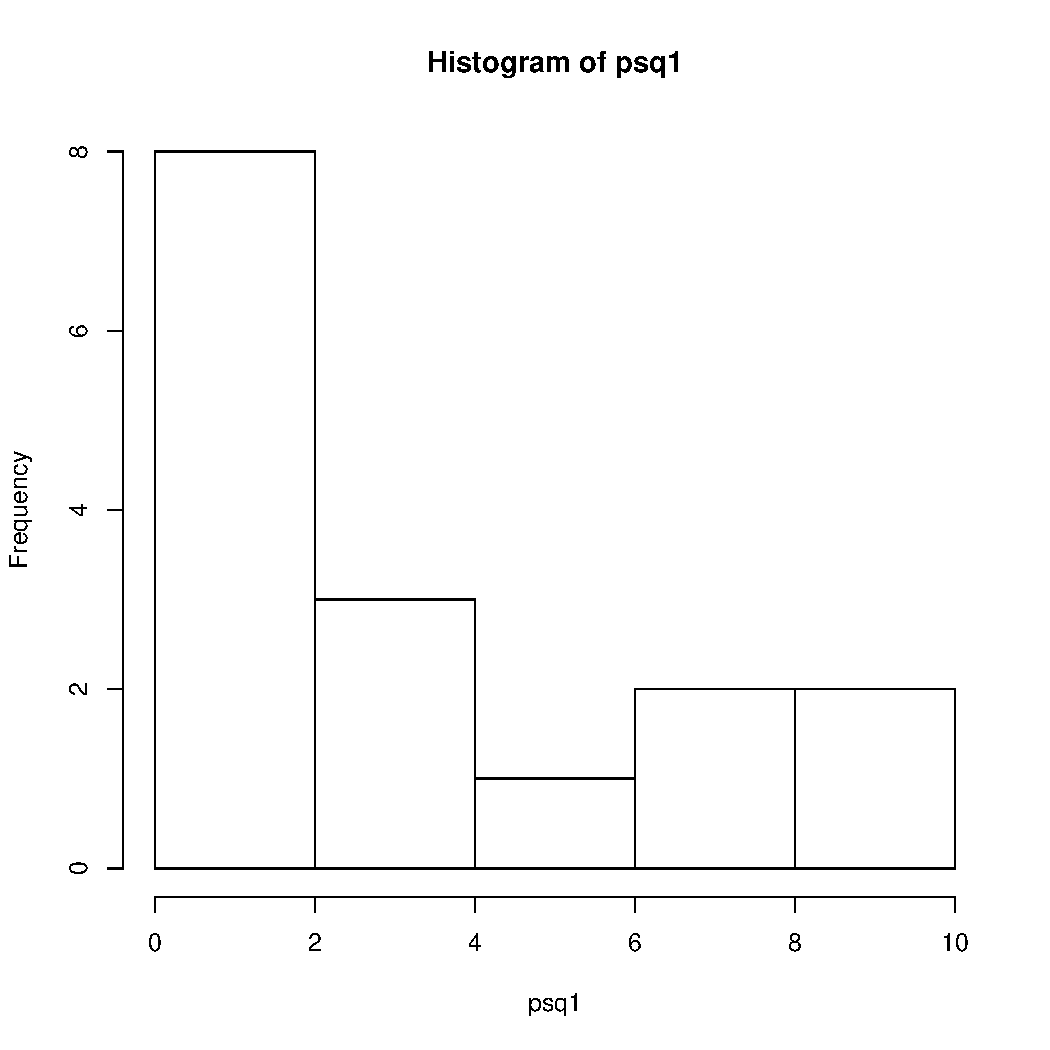
\includegraphics[width=0.3\textwidth]{figuras/parte1/post_sigma1.pdf}}
	\subfigure[]{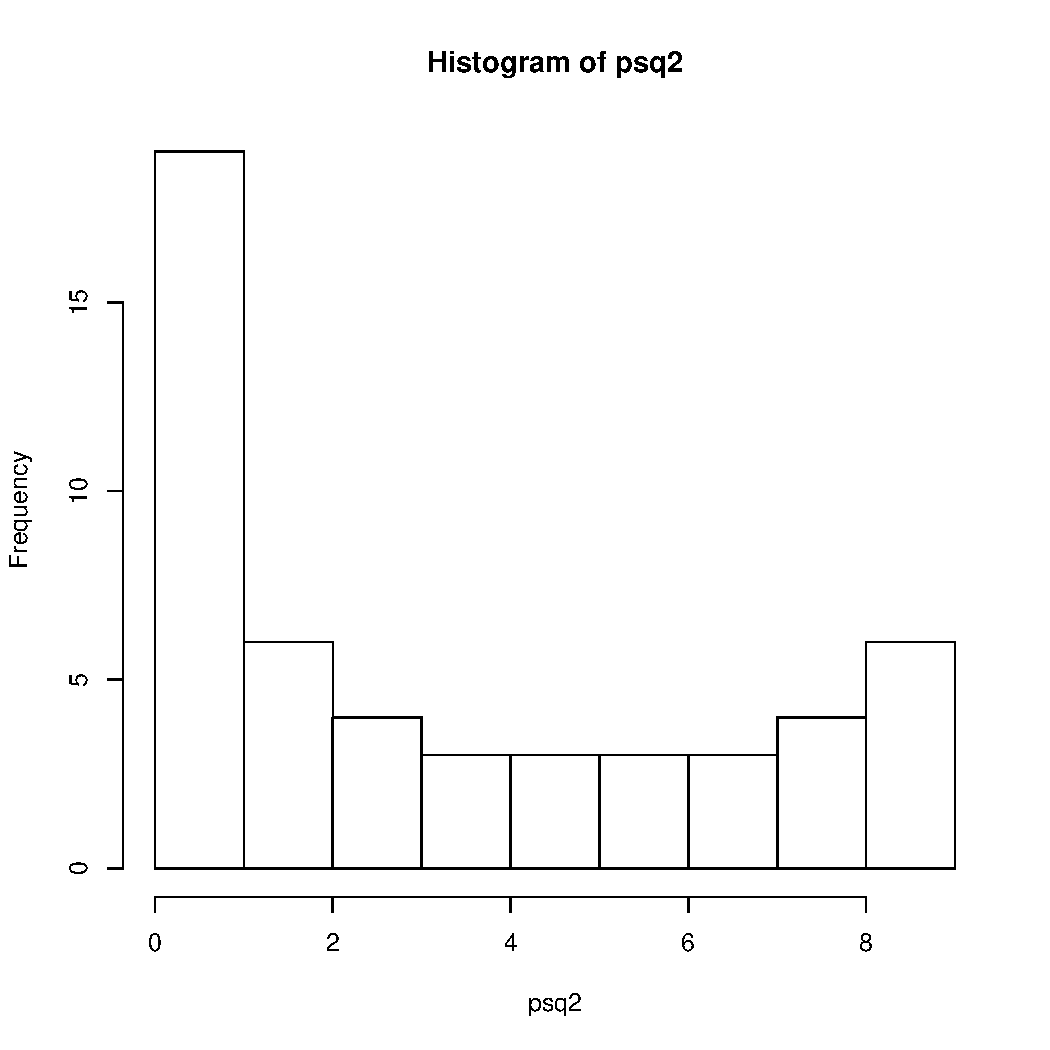
\includegraphics[width=0.3\textwidth]{figuras/parte1/post_sigma2.pdf}} 
	\subfigure[]{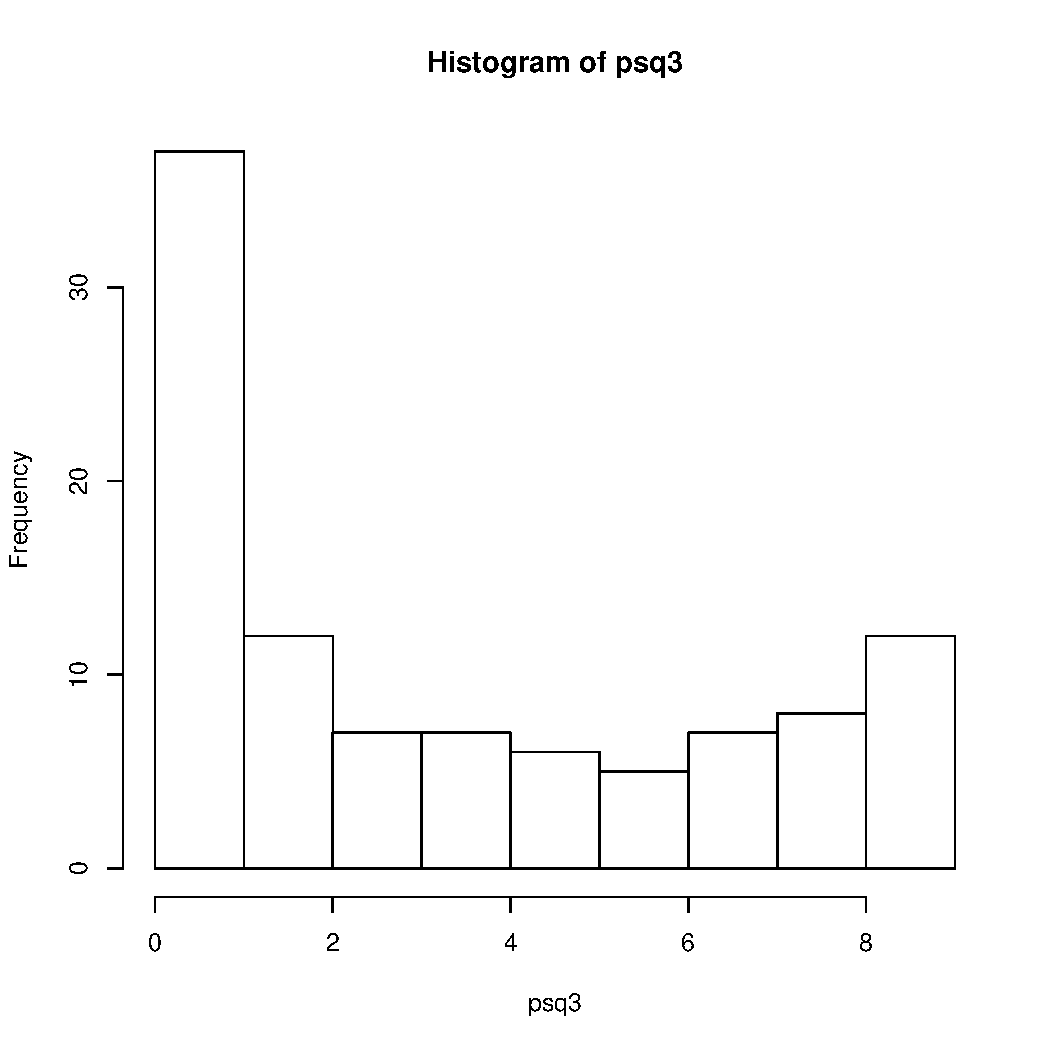
\includegraphics[width=0.3\textwidth]{figuras/parte1/post_sigma3.pdf}} 
	\caption{Posteriori de sigma}
	\label{fig:post_sigma}
\end{figure}

\begin{figure}[!htb]
	\centering
	\subfigure[]{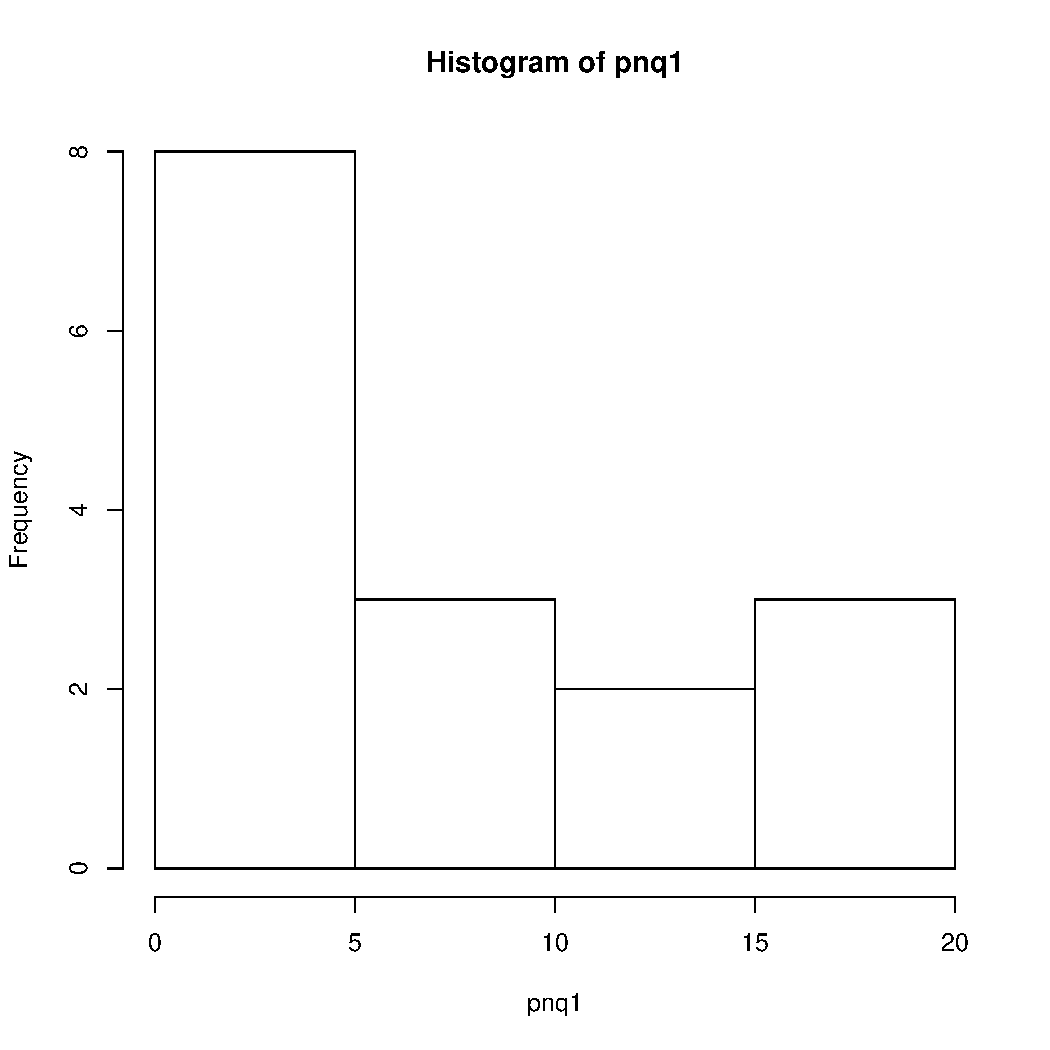
\includegraphics[width=0.3\textwidth]{figuras/parte1/post_nu1.pdf}}
	\subfigure[]{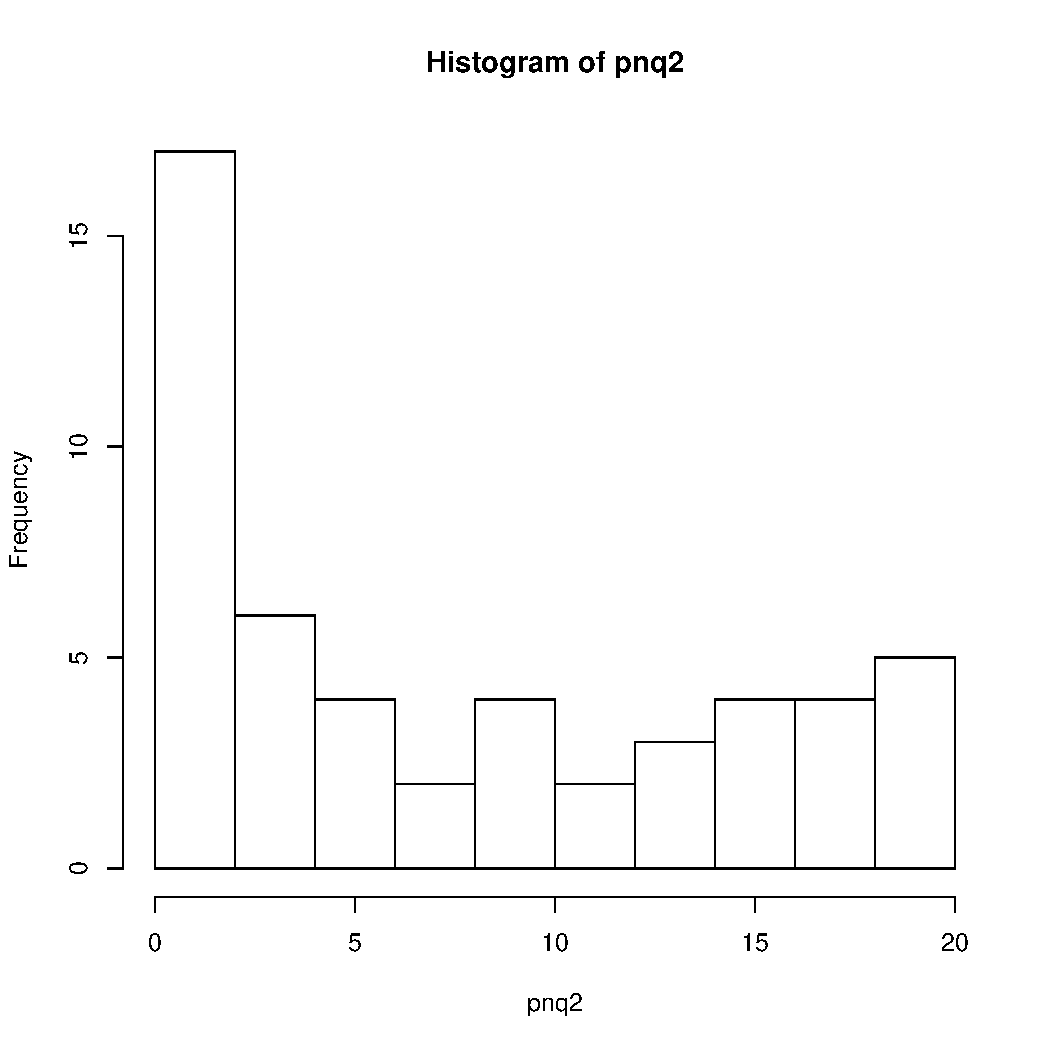
\includegraphics[width=0.3\textwidth]{figuras/parte1/post_nu2.pdf}} 
	\subfigure[]{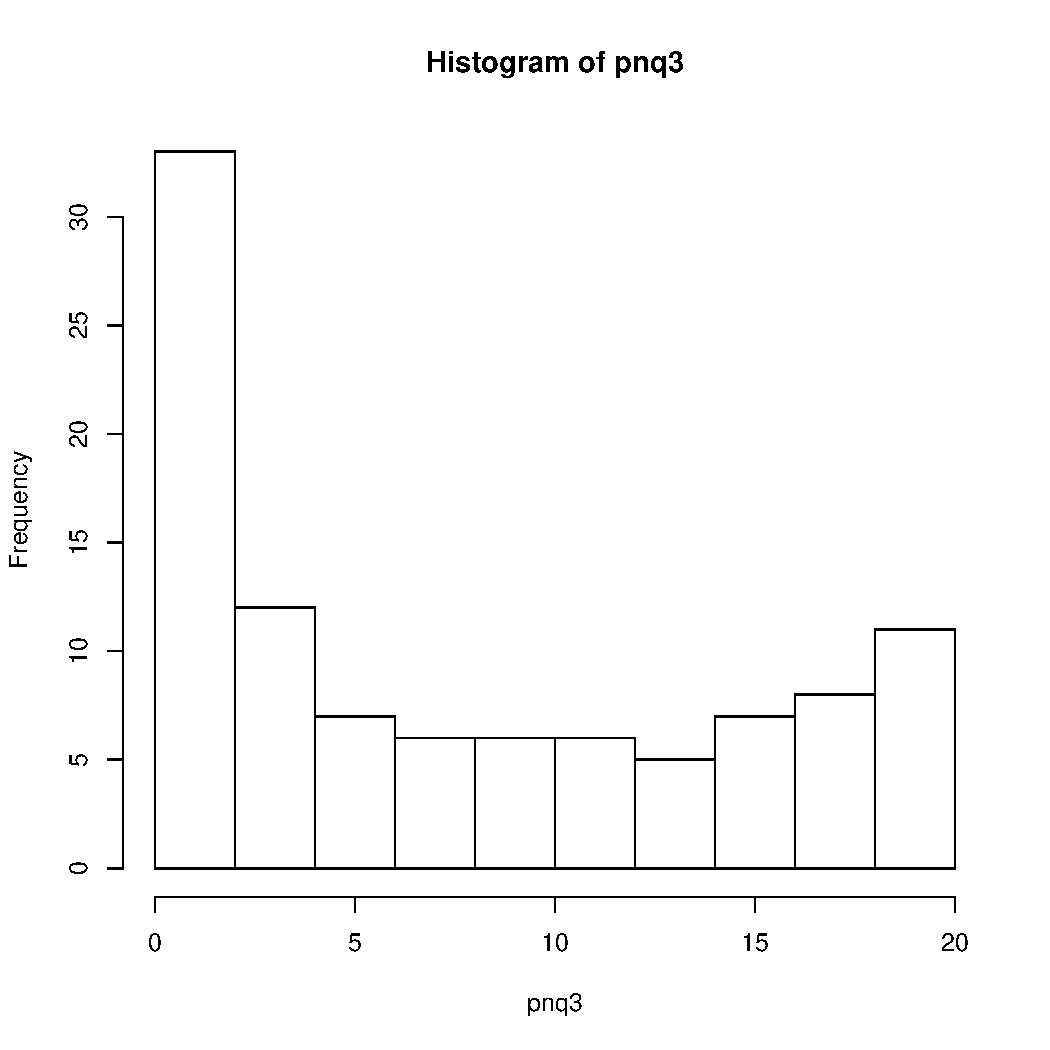
\includegraphics[width=0.3\textwidth]{figuras/parte1/post_nu3.pdf}} 
	\caption{Posteriori de nu}
	\label{fig:post_nu}
\end{figure}

\section*{\Large O Método da Reamostragem Ponderada}

%Texto descrevendo o método e como foi feita neste trabalho a geração de variáveis aleatórias da distribuição de interesse usando este mesmo método.

\section*{\Large O Método de Monte Carlo via Cadeias de Markov}

%Texto descrevendo o método e como foi feita neste trabalho a geração de variáveis aleatórias da distribuição de interesse usando este mesmo método, bem como o amostrador selecionado (possivelmente Gibbs ou outro que for de melhor uso para todo o grupo).

\bibliographystyle{unsrt}
%\bibliography{arquivo.bib}

\end{document}